\documentclass[main.tex]{subfiles}
\begin{document}


\section{Локальность}\label{ch14}

Замена гармонических осцилляторов гармоническими ротаторами может быть первым шагом к получению гамильтониана, который, с одной стороны, описывает детерминированные процессы, а с другой стороны все еще подчиняется ограниченности снизу. И все же придется раскошелиться. Мы изменили правила коммутации между операторами координат, называемыми $x$, и операторами импульса $p$. Если бы мы применили это к теориям поля, нам было бы трудно разложить поля на гармонические моды. Эти режимы больше не будут коммутировать друг с другом, и это станет серьезным ударом по концепции локальности.

Мы также видели, как можно построить гамильтониан, начиная с любой детерминированной системы, включая системы, которые являются полностью локальными в обычном смысле. Если время непрерывно, этот гамильтониан имеет тенденцию принимать форму (\ref{12.18}), которая не имеет ни нижней, ни верхней границы, но, похоже, является локальной. Напротив, гамильтонианы моделей с дискретным временем, таких как (\ref{2.8}), (\ref{2.26}), (\ref{2.27}) и (\ref{12.10}) объединяет их ограниченность, но они выражаются через операторы эволюции в довольно большие моменты времени $t = n\delta t$. Для моделей клеточных автоматов, обсуждаемых в разд. \ref{ch5.1} и \ref{ch21}, оператор эволюции в течение $n$ временных шагов, включает взаимодействия между соседями, которые находятся на расстоянии $n$ шагов друг от друга. Если вместо этого мы хотим ограничиться локальными выражениями, это означает, что при определении $H$ потребуется ввести отсечение, но это допустимо только в том случае, если соответствующие суммы сходятся достаточно быстро. Кажется, что это сочетание требования позитивности и локальности, которое часто трудно соблюдать.

Можно ли избежать этого конфликта? Должны ли мы искать разные модели или искать разные методы применения, которые используются во всех моделях? Настоящее понимание автора заключается в том, что мы должны поставить ограничения на модели, к которым мы можем применить наши теории. Различные модели будут обсуждаться позже (раздел \ref{ch9.2}). Давайте здесь сосредоточимся на природе конфликта.

В первой части, раздела \ref{2.1} мы ввели понятие шаблонов. Давайте посмотрим, что произойдет, когда мы наложим дополнительное ограничение на шаблоны: рассмотрим только те состояния шаблонов, которые медленно меняются во времени. Мы предполагаем, что временная зависимость в шаблонах намного медленнее, чем фундаментальный временной интервал $\delta t$ в законе онтологической эволюции. Это означает, что мы рассматриваем только те элементы Гильбертова пространства, в которых собственное значение $E$ матрицы $H$ лежит в интервале $|E|\le\frac 1 2 \Lambda$, или, когда мы добавляем нашу свободную постоянную к уровням энергии, мы навязываем

\begin{equation}\label{14.1}
	0\le E\le\Lambda
\end{equation}

Состояния, составленные в виде суперпозиций этих собственных значений энергии, покажут вероятности $|\langle ont\mid\psi(t)\rangle|^2$, чья зависимость от времени содержит только члены $e^{i\omega t}$ с $|\omega|\le\Lambda$. Шаблоны подчиняющиеся неравенству (\ref{14.1}) будет называться медленными шаблонами.

Рекомендуется, однако, воздержаться от использования медленных шаблонов; в классических состояниях, энергии могут легко достигать значений выше энергии Планка (кинетическая энергия небольшого пассажирского самолета на крейсерской скорости), и для этого потребуются более быстрые шаблоны.

На рисунке \ref{i14.1}a показано приближение, полученное для гамильтониана, в случае использования разложения (\ref{2.8}) с плавным обрезанием. Мы ввели коэффициент подавления $e^{-k/R}$ для k-го члена (на рисунке $R = 30$). Что происходит, когда мы используем это приближение для гамильтониана?

Во-первых, он уже не совсем локален. В клеточном автомате, где у нас есть только взаимодействия ближайших соседей, гамильтониан будет показывать «призрачные взаимодействия» между соседями на расстоянии $k$ единиц друг от друга, предполагая, что k-й член содержит оператор эволюции $U (\pm k\delta t)$. С учетом коэффициента подавления мы ожидаем, что гамильтониан будет иметь нелокальные особенности на масштабах расстояний порядка $R\delta tc$, где $c$ - максимальная скорость передачи информации в автомате, поскольку экспоненциальный коэффициент подавления сильно подавляет эффекты, распространяющиеся дальше.

С другой стороны, если мы используем коэффициент подавления, самые низкие энергетические состояния в спектре будут изменены, см. Стрелку на Рис. \ref{i14.1}a. К сожалению, это именно физически самая важная область, близкая к состоянию вакуума (состояние с самой низкой энергией). Нетрудно оценить степень деформации, близкой к началу. Сумма с отсечкой может быть оценена точно. Для больших значений среза $R$ и $0 <\omega <\pi$ аппроксимация $\omega_{approx}$ для истинных собственных значений $\omega$ гамильтониана будет выглядеть так:

\begin{equation}\label{14.2}
	\begin{aligned} \omega_{\text {approx }} &=\pi-2 \sum_{n=1}^{\infty} \frac{\sin (n \omega) e^{-n / R}}{n}=2 \arctan \left(\frac{e^{1 / R}-\cos \omega}{\sin \omega}\right) \\ &=2 \arctan \left(\frac{1-\cos \omega+1 / R}{\sin \omega}\right)=2 \arctan \left(\frac{\sin \omega}{1+\cos \omega}+\frac{1 / R}{\sin \omega}\right) \end{aligned}
\end{equation}

где мы заменили $e^{1 / R}$ на $1+1/R$, поскольку $R$ велико и произвольно.
 
Записав $\frac{\sin \alpha}{1+\cos\alpha} = \tan\frac 1 2 \alpha$, мы видим, что приближение становится точным в пределе $R \rightarrow\infty$. Нас интересуют состояния, близкие к вакууму, имеющие малую, но положительная энергия $H = \alpha$. Тогда при конечном $R$ обрезание в $R$ заменяет собственные значения $H$ гамильтониана $H_\mathrm{op}$ на

\begin{equation}\label{14.3}
	H \rightarrow H + \frac{2}{RH}
\end{equation}
            
который имеет минимум при $H_0 \approx\sqrt{2 / R}$, где значение минимума равно $H \approx 2\sqrt{2 / R}$. Это приемлемо только если

\begin{equation}\label{14.4}
	R \gg M_{\mathrm{Pl}} /\left\langle H_{\mathrm{op}}\right\rangle^{2}
\end{equation}

\begin{figure}[ht]
\begin{center}
\scalebox{0.4}{
   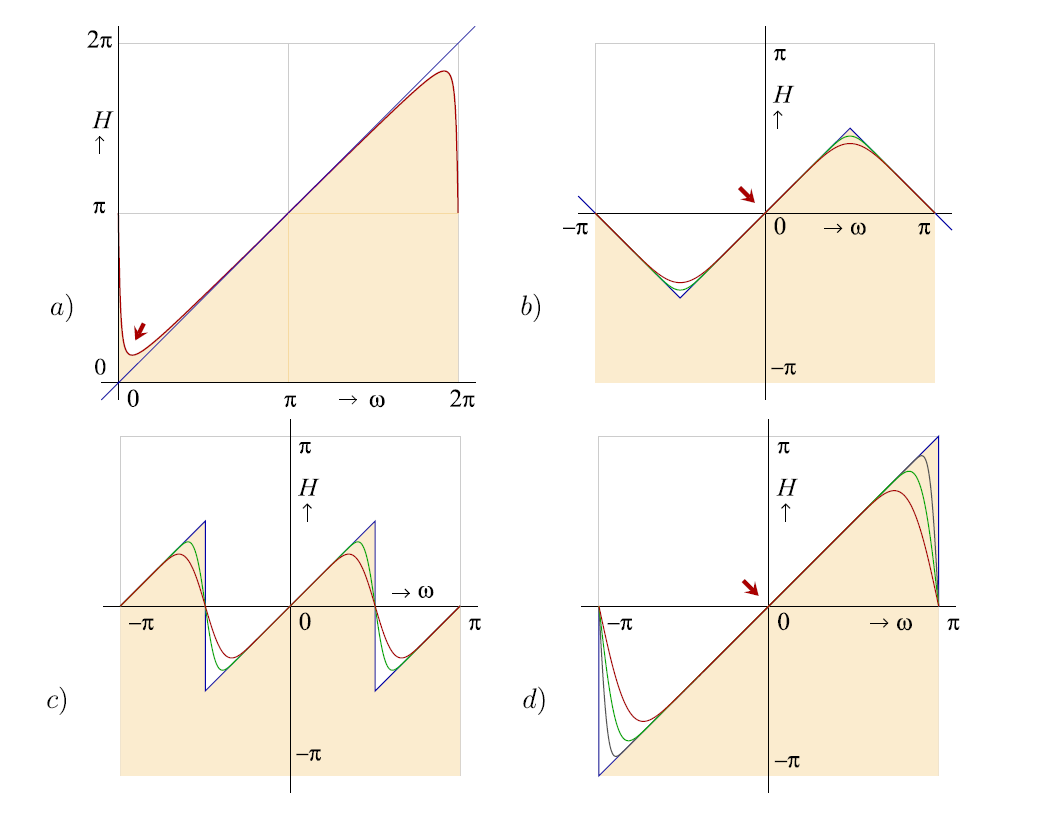
\includegraphics{images/img_14_1.png}
}
\caption{
\label{i14.1} Спектр гамильтониана в различных разложениях. \textbf{a.} Разложение Фурье (\ref{2.8}) с коэффициентом подавления R = 30. Наиболее важный участок вблизи вакуума, показанный стрелкой, максимально искажен коэффициентом подавления. \textbf{b.} Используя разложение (\ref{14.6}) для $\arcsin(z)$, получить наиболее точное разложение для $H$ вблизи центра спектра. Кривые показаны для R = 9 и R = 31. \textbf{c.} Результат после умножения на $\cos\omega/|\cos\omega|$. Показанные кривые доходят до степеней 13 и 41. \textbf{d.} Растяжение предыдущей кривой с коэффициентом 2 затем удаляет нежелательные состояния (см. Текст). Показанные значения: 10, 30 и 120 (разница между цифрами и точками, прямая линия в центре приближается гораздо точнее)}
\end {center}
\end {figure}

 
Здесь $M_{Pl}$ - это «масса Планка», или что бы то ни было, обратное элементарной шкале времени в модели. Поэтому этот радиус обрезания R должен быть выбран очень большим, чтобы точное квантовое описание нашей локальной модели действительно приводило к нелокальности в гамильтониане.

Таким образом, если мы хотим, чтобы гамильтониан правильно представлял поведение вблизи вакуума, чтобы шкалы времени порядка $T$ были описаны правильно, то гамильтониан, генерируемый моделью, будет нелокальным на гораздо больших расстояниях порядка $T^2M_{Pl}$. По-видимому, детерминированный автомат генерирует квантовое поведение, но квантовый гамильтониан имеет ложные нелокальные взаимодействия.

Нетрудно заметить, что конфликт между локальностью и положительностью, с которым мы столкнулись, вызван тем фактом, что спектр энергии должен был быть выбран так, чтобы скачок $\theta$ происходил при $\omega = 0$, именно там, где мы имеем вакуумное состояние (см. рис. \ref{i14.1}а). Коэффициенты Фурье функции со скачком $\theta$ всегда будут сходиться очень медленно, и чем острее мы хотим, чтобы этот разрыв воспроизводился нашим гамильтонианом, тем больше нужно коэффициентов Фурье. 

Действительно, индуцированная нелокальность будет намного больше, чем размер системы, которую мы могли бы изучить. Подчеркнем, что эта нелокальность чисто умозрительна; физика самого автомата довольно локальна, так как только непосредственно соседние ячейки влияют друг на друга. Однако полученная квантовая механика не похожа на то, что мы видим в физическом мире, где гамильтониан можно рассматривать как интеграл по плотности Гамильтона $\mathcal H (\vec x)$, где $\left[\mathcal H (\vec x),\mathcal H (\vec x')\right] = 0$ при $| \vec x - \vec x'| > \varepsilon > 0$. В стандартных квантовых теориях поля это $\varepsilon$ стремится к нулю. Если он простирается на миллионы клеток , то  будет неприемлемо, если это расстояние нельзя обнаружить в современных экспериментах. Очевидно, что лучшую стратегию еще предстоит найти.

Наше лучшее предположение в настоящее время для решения этой проблемы - это вторичное квантование, которое было введено в разделе \ref{ch9.2}, и мы продолжим мысль в разделах \ref{ch20.3} и \ref{ch22.1}. Здесь мы просто упоминаем, что вторичное квантование позволит нам иметь наиболее важные физические свойства в центральной области этого спектра, а не по краям, см. стрелку на рис. \ref{i14.1}b. В этом регионе наши эффективные гамильтонианы могут быть очень точными, но в то же время локальными. Предположим, что мы разлагаем гамильтониан в терминах коэффициентов Фурье, которые ведут себя как

\begin{equation}\label{14.5}
	(\sin \omega)^{n}=(i / 2)^{n}(U(\delta t)-U(-\delta t))^{n}
\end{equation}

с ограничением по степеням $n$. Для малых $\omega$, наиболее точным приближением может быть

\begin{equation}\label{14.6}
	\omega=\sum_{n=0}^{(R-1) / 2} a_{n}(\sin \omega)^{2 n+1}
\end{equation}

где $a_n = 1, \frac 1 6, \frac{3}{40}, \frac{5}{112},\ldots$ - коэффициенты разложения $\arcsin(z)$ по степеням z. Если мы продолжим до степени $R$, мы получим очень быстро сходящееся выражение для энергии вблизи центра спектра, где $\omega$ мало. Если мы используем эту часть спектра, погрешность в гамильтониане будет иметь порядок $(\omega\delta t)^{R+2}$, так что достаточно лишь нескольких соседей, чтобы дать достаточно точный гамильтониан.

Тем не менее, рис. \ref{i14.1}b все еще не совсем то, что мы хотим. Для всех состояний, у которых $\omega$ близко к $\pm\pi$, энергии также низки, хотя это не те состояния, которые следует включать, в частности, когда возмущения добавляются для создания взаимодействий. Чтобы удалить эти состояния, нам нужны разложения Фурье, которые генерируют кривые на рис. \ref{i14.1}d. Здесь состояния с $\omega\approx\pi$ по-прежнему вносят свой вклад, что неизбежно, потому что, действительно, мы не можем избежать там скачка $\theta$, но поскольку линии сейчас намного круче в этом месте, состояниями при $\omega = \pm\pi$ можно безопасно пренебречь; лучшее выражение, которое мы можем сгенерировать, будет иметь плотность паразитных состояний, которая падает как $1/\sqrt{R}$, умноженная на плотность разрешенных состояний. Как можно генерировать эти разложения Фурье?

Вернемся к фиг.\ref{i14.1}b и заметим, что дифференцирование по $\omega$ дает нам разложение Фурье функции $\theta$. Умножая это на оригинал, мы получим функции рис. \ref{i14.1}c. Самый простой способ увидеть, что происходит, - это заметить, что мы умножаем предельную кривую (зигзагообразную линию в \ref{i14.1}b) на $\cos\omega/|\cos\omega|$, где знаменатель расширяется по степеням $\sin(\omega)$. Затем получаем

\begin{equation}\label{14.7}
	H(\omega)=\cos \omega \sum_{k=0}^{(R-1) / 2} b_{k}(\sin \omega)^{2 k+1}
\end{equation}

где $\sum_k b_k x^{2k+1}$, с $b_k = 1, \frac 2 3, \frac{8}{15}, \frac{16}{35}, \frac{128}{315},\ldots$ - степенной ряд для

\begin{equation}\label{14.8}
	(\arcsin z) / \sqrt{1-z^{2}}
\end{equation}
   
в степенях $z$.

Наконец, поскольку график \ref{i14.1}c является периодическим с периодом $\pi$, мы можем растянуть его, умножив $\omega$ на 2. Это дает рис. \ref{i14.1}d, где предельная кривая аппроксимируется

\begin{equation}\label{14.9}
	H(\omega)=\sin \omega \sum_{k=0}^{R-1} b_{k}((1-\cos \omega) / 2)^{k}
\end{equation}

с такими же коэффициентами $b_k$. Таким образом, теперь именно это уравнение мы используем для определения оператора $H$ из оператора эволюции одношагового $U = U (\delta t)$. Используя $\bar U$ для обозначения обратного $\bar U = U (-\delta t) = U^{-1}$, подставим в уравнение. (\ref{14.9}):

\begin{equation}\label{14.10}
	\sin \omega=\frac{i}{2}(U-\bar{U}), \quad(1-\cos \omega) / 2=\frac{1}{4}(2-U-\bar{U})
\end{equation}

Уловка, которую мы можем затем применить, состоит в том, чтобы рассматривать состояния с отрицательной энергией как  античастицы после того, как мы применяем вторичное квантование. Этот очень важный шаг, который мы в первую очередь применим к фермионам, представлен в следующем разделе, а взаимодействие отложено до раздела \ref{22.1}.

\end{document}